\documentclass{standalone}
\usepackage{tikz}
\usetikzlibrary{intersections}
\renewcommand{\familydefault}{\sfdefault}

\usepackage{
tikz,
pgfplots,
}

\usetikzlibrary{
calc
}

%===================================================
%SOLUTION STARTS HERE - comment out to see change
%===================================================
\newcommand{\mybasiclinewidth}{very thick}
%source is page 126 in the manual
\tikzset{
every picture/.style={
\mybasiclinewidth} %or use: "`line width=1 pt,"<-- note:if you write line width, you must use a value with unit
}
\pgfplotsset{
every axis/.append style={
\mybasiclinewidth,
grid style={
    \mybasiclinewidth,
},
tick style={
    \mybasiclinewidth,
},
},
}
%===================================================
%SOLUTION ENDS HERE - comment out to see change
%===================================================

\begin{document}
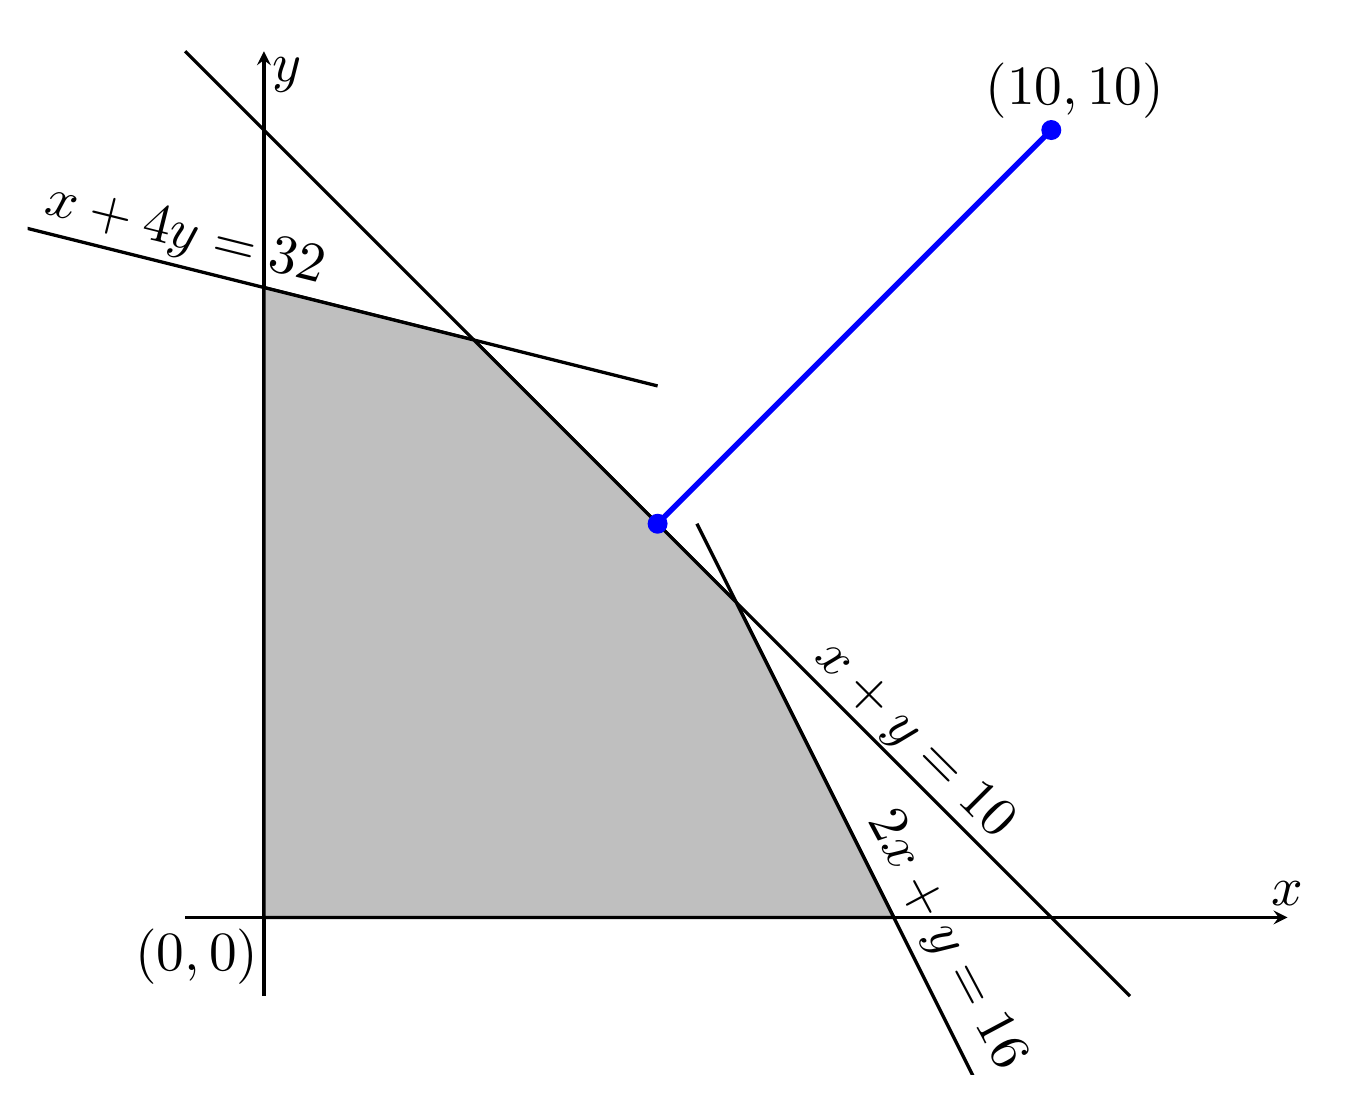
\begin{tikzpicture}[>=stealth]
%   \draw [fill = blue, opacity = .3] plot [smooth cycle] coordinates {(0,0) (1,1) (2,1) (3,-1) (0,-1)};
%   \draw [fill = red, opacity = .3] plot [smooth cycle] coordinates {(2,0) (3,2) (4, 1.5) (4, -1)};
%   \draw [fill = green, opacity = .3] plot [smooth cycle] coordinates {(1,2) (3,.3) (0, .1)};

%   \draw plot [smooth cycle] coordinates {(0,0) (1,1) (2,1) (3,-1) (0,-1)};
%   \draw  plot [smooth cycle] coordinates {(2,0) (3,2) (4, 1.5) (4, -1)};
%   \draw  plot [smooth cycle] coordinates {(1,2) (3,.3) (0, .1)};

  % \begin{scope}[xshift = 6cm]
  % \draw [fill = gray!50] (0, 0) -- (2, -.81) -- (3, 1) -- (2, 2) -- (.5, 2) -- (0, 1) -- cycle;
  
  % \def\k{5.25}
  % \def\ax{2.65}
  % \def\bx{3.4}
  % \def\ay{\d*(\ax - 3) + 1}
  % \draw [thick, dashed, opacity = .8, green] ({\ax}, {\k*(\ax - 3) + 1}) -- ({\bx}, {\k*(\bx - 3) + 1});
  % \draw [thick, dashed, opacity = .8, cyan] ({\ax +1}, {\k*(\ax - 3) + 1}) -- ({\bx+1}, {\k*(\bx - 3) + 1});
  % \draw [thick, dashed, opacity = .8, blue] ({\ax +2}, {\k*(\ax - 3) + 1}) -- ({\bx+2}, {\k*(\bx - 3) + 1});
  % \draw [thick, dashed, opacity = .8, yellow] ({\ax - 1}, {\k*(\ax - 3) + 1}) -- ({\bx-1}, {\k*(\bx - 3) + 1});
  % \draw [thick, dashed, opacity = .8, orange] ({\ax - 2}, {\k*(\ax - 3) + 1}) -- ({\bx-2}, {\k*(\bx - 3) + 1});
  % \draw [thick, dashed, opacity = .8, red!50!orange] ({\ax - 3}, {\k*(\ax - 3) + 1}) -- ({\bx-3}, {\k*(\bx - 3) + 1});
  % \draw [thick, dashed, opacity = .8, red] ({\ax - 4}, {\k*(\ax - 3) + 1}) -- ({\bx-4}, {\k*(\bx - 3) + 1});
  % \draw [->] (3, 1) -- (3 + .3*\k, 1 - .3);

  % \draw [fill = red, draw = red] (0, 1 ) circle (1pt);

  % \node at (1.5, 0.4) {feasible set $\mathcal{X}$};
  % \node at (1.5, 2.4) {Linear Programming};
  % \node at (2.7, 1) {$\mathbf{x}_0$};
  % \node at (2.5, 1) {$\mathbf - 2{x}_0$};
  % \node at (2.5, 1) {$\mathbf - 2{x}_0$};
  % \node at (2.5, 1) {$\mathbf - 2{x}_0$};
  % \node at (.3, 1) {$\mathbf{x}_1$};
  % \node at (4.3, 1) {$-\mathbf{c}$};
  % % \draw (-1, .5) -- (3, -1.5);
  % % \draw (1.5, -2) -- (3.5, 2);
  % % \draw (-.5, .75) -- (3, 2.5);
  % % \draw (0, -1) -- (0, 2);
  % % \draw (3.5, .5) -- (1.5, 2.5);

  % \end{scope}

  % axes 
  \clip (-3, -2) rectangle (13.5, 11.3);
  \def\s{1}
  \draw [->] (-\s, 0) -- (13*\s, 0);
  \node [scale = 2] at (13, .3) {$x$};
  \draw [->] (0, -\s) -- (0, 11);
  \node [scale = 2] at (.3, 10.7) {$y$};
  \draw (-1, 11) -- (11, -1); 
  \node [rotate = -45, scale = 2] at (8.25, 2.25) {$x + y  = 10$};

  % \draw (-3, 9) -- (10, -4);
  % \node [rotate = -45, scale = 2] at (2.75, 2.75) {$x + y  = 6$};

  \draw (5.5, 5) -- (10, -4);
  \node [rotate = -62, scale = 2] at ( 8.65, -.3) {$2x + y = 16$};

  \draw (-4, 9) -- (5, 6.75);
  \node [rotate = -14, scale = 2] at (-1, 8.65) {$x + 4y = 32$};

  % \node [rotate = -60, scale = 2] at (9.4, 6) {$5x + 3y = b$ (a constant)};


  \draw [fill = gray!50] (0, 0) -- (8, 0) -- (6, 4) -- (8/3, 22/3) --(0, 8) -- cycle;

  % \draw [line width = 1mm, opacity = .8, dashed, red] (13, -1) -- (32/5, 10);
  % \draw [line width = 1mm, opacity = .8, dashed, orange] (11, -1) -- (22/5, 10);
  % \draw [line width = 1mm, opacity = .8, dashed, yellow!50!black] (9, -1) -- (12/5, 10);
  % \draw [line width = 1mm, opacity = .8, dashed, green] (7, -1) -- ( 2/5, 10);
  % \draw [line width = 1mm, opacity = .8, dashed, cyan] (5, -1) -- ( 2/5 - 2, 10);
  % \draw [line width = 1mm, opacity = .8, dashed, blue] (3, -1) -- ( 2/5 - 4, 10);
  % \draw [line width = 1mm, opacity = .8, dashed, blue!80!black] (1, -1) -- ( 2/5 - 6, 10);

  \draw [fill = blue, draw = blue] (10, 10 ) circle (3pt);
  \draw [fill = blue, draw = blue] (5, 5 ) circle (3pt);
  \draw [blue, line width = 2] (10, 10) -- (5, 5);
  % \draw [fill = black, draw = black] (0, 0 ) circle (3pt);
  % \node [scale = 2, rotate = -45] at (4, 4) {feasible set $\mathcal{X}$};
  \node [scale = 2] at (-.85, -.5) {$(0, 0)$};
  \node [scale = 2] at (10.3, 10.5) {$(10, 10)$};
  % \node [scale = 2] at (4.5, 4.5) {$(5, 5)$};

\end{tikzpicture}
\end{document} 